\documentclass{article}
\usepackage{amssymb, amsmath}
\usepackage[utf8]{inputenc}
%\usepackage{fullpage}
\usepackage[parfill]{parskip}
\usepackage{graphicx}
\usepackage{ifthen}

\DeclareGraphicsExtensions{.pdf,.png,.jpg}

\begin{document}
%	\begin{center}
%		\textbf{Prueba de texto: Intención}
%	\end{center}	
%Desarrollos fundamentales para el libro de cálculo.

Esto es un bosquejo de lo que será la parte introductoria del libro de cálculo a ser publicado bajo licencia Creative Commons. 

El cálculo posee dos símbolos particulares que definen su esencia. La idea general detrás de ellos, sin embargo, no es nada complicada: \\
 
\begin{center}
$d$ significa "una pequeña parte de" \\
$\int$ significa "suma de todas las pequeñas partes" \\
\end{center}


Por lo tanto, $dx$ significa "una pequeña parte de $x$, y $du$ significa "una pequeña parte de $u$. Como veremos más adelante, lo de "pequeño" viene a ser para algo infinitamente pequeño.

Por su parte, el símbolo $\int$ es como una $S$ larga, y bien podría interpretarse como un tipo especial de suma. Significa "la suma de todas las partes pequeñas de". Por ejemplo, $\int dx$  es la suma de todas las partes pequeñas de $x$, y $\int dt$ es la suma de todas las partes pequeñas de $t$.

\newpage

Para llegar al concepto de derivada nos valdremos de un cuadrado cualquiera. Supongamos que lo estiramos con las manos un poco. El cuadrado conserva sus proporciones, y luego podemos comparar la forma final con la forma inicial. Llamamos x al tamaño que tenía cada lado al principio, dx al aumento realizado, y x + dx al tamaño final de cualquiera de los lados. Si aumentas por un punto el ancho, entonces el alto aumentará en una línea completa del tamaño de x. \\

	\begin{center}
	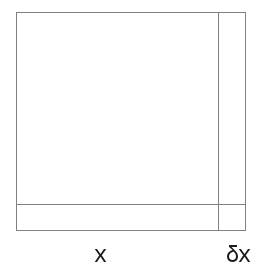
\includegraphics[width=5cm]{deriv_area_square}
	\end{center}
	
	\begin{align*}
		y &= x^2 \\
		y + \delta y &= (x + \delta x) ^ 2 \\
		y + \delta y &= x^2 + 2x\delta x + (\delta x)^2 \\
		\delta y &= 2x\delta x + \delta x \\
		\frac{\delta y}{\delta x} &= 2x + \delta x
	\end{align*}

Un poco más formalmente, podemos decir que la derivada de la función del área del cuadrado es lo que obtienes si le restas el resultado inicial al resultado final, y divides todo entre un tamaño de cambio infinitamente pequeño. Esto se escribe en notación de límites de la siguiente manera: 

	\begin{align*}
		f'(x) &= \inf_{\Delta x \to 0}
			\frac{f(x + \Delta x) - f(x)}{\Delta x}
	\end{align*}

\newpage

El caso del área del rectángulo es un poco más complejo, ya que ahora no todos los lados son iguales. Dos tienen un largo "x", y dos un largo "y". Si denominamos al área "z", entonces tenemos que las dos derivadas parciales son la misma expresión derivada en base a la variable que nos interesa (hay casos más complicados, pero por ahora esto es suficiente). \\

	\begin{center}
		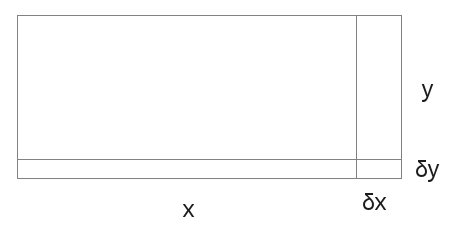
\includegraphics[keepaspectratio=true, width=5cm]{deriv_area_rectangle}
	\end{center}

	\begin{align*}
		z &= xy \\
		\frac{\partial z}{\partial x} &= \frac{d(xy)}{dx} = x\delta x \\
		\frac{\partial z}{\partial y} &= \frac{d(xy)}{dy} = y\delta y
	\end{align*}
	
	\begin{align*}
		f_x(x, y) &= \inf_{\Delta x \to 0}
			\frac{f(x+\Delta x, y) - f(x, y)}{\Delta x} \\
		f_y(x, y) &= \inf_{\Delta y \to 0}
			\frac{f(x, y+\Delta y) - f(x, y)}{\Delta y} \\
	\end{align*}
	
\end{document}
